\documentclass[conference]{IEEEtran}
\IEEEoverridecommandlockouts
% The preceding line is only needed to identify funding in the first footnote. If that is unneeded, please comment it out.
\usepackage{biblatex}
\usepackage{amsmath,amssymb,amsfonts}
\usepackage{algorithmic}
\usepackage{graphicx}
\usepackage{textcomp}
\usepackage{xcolor}
\def\BibTeX{{\rm B\kern-.05em{\sc i\kern-.025em b}\kern-.08em
    T\kern-.1667em\lower.7ex\hbox{E}\kern-.125emX}}

\addbibresource{citations.bib}

\begin{document}

\title{Graph Databases for Use with Timeseries IoT Datasets}

\author{\IEEEauthorblockN{Colter Snyder}
\IEEEauthorblockA{\textit{Department of Computer Science} \\
\textit{Colorado School of Mines}\\
Golden, Colorado, USA \\
csnyder1@mines.edu}
}

\maketitle

\begin{abstract}
The wide spread proliferation of Internet of Things (IoT) devices
have brought up many questions and concerns about their security
and what they do with data. Many solutions have appeared using 
various solutions such as IoT Inspector \cite{IoTInspector}. 
However, these solutions don't make use of the unique capabilities
and efficiencies that graph databases provide. This paper seeks
to use a graph database in order to answer challenging questions 
about IoT devices particularly within the realm of timeseries datasets.
\end{abstract}

\begin{IEEEkeywords}
IoT, Graphical Databases, Database Systems, Systems
\end{IEEEkeywords}

\section{Introduction}
Smart homes are everywhere now adays, from lights to door locks, TVs to speakers.
It seems that these devices, which are refered to by their collective as Internet of Things or IoT devices, are in every home.
With all these new devices come a whole slew of concerns about privacy and security \cite{IoTInspector}.
There are many papers that explore these concerns, what this paper seeks to persue is how to efficiently analyze
data collected from these devices such that people may infer various aspects about their devices. In particular,
this paper seeks to see what what info can be garnered from timeseries datasets. Such aspects could include
anything from what the device is doing to answering if a device is attacking the network and how.

It was decided that using a graph database could provide answers to these questions
more efficiently and easily than a relational database. The primary advantage for use in this paper
is the fact that graph databases are great for use with densely connected data \cite{GraphSurvey}.
On top of this, they are very quick to query and will give a result relatively quickly compared to
other solutions \cite{GraphSurvey}. In particular, the use for home users and smaller networks was 
examined by asking what queries could be run on a smaller dataset as well as what would be reasonable
for a home user as far as time and efficiency.

The hope of this paper is to provide basic evidence to determine if graph databases are truly a good solution 
for these users and see if they are able to answer questions that these users would want to ask about their 
networks. For instance, we explore finding whether or not certain attacks had taken place on these systems,
a question that would likely interest anyone running a network of IoT devices. What this paper is not, however,
is a comprehensive review of this method against all the existing methods out there. While this would be
undoubtadly useful, due to constraints and limitations faced by the author this has been left up to future work.

\section{Related Works}
There are many current systems that implement different components of the general idea of graphical databases for
IoT device management andanomoly detection, but none put these components together. \textit{IoT Inspector} is a great
tool that performs the task of monitoring using a form of a relational database, but not a graphical one \cite{IoTInspector}.
The authors of \textit{The Graph of Things} created such a system for aggregating IoT devices worldwide \cite{GraphofThings}; 
However, these systems are not built for small networks or home users. What this paper seeks to explore is what questions
can a graph database answer for these smaller networks, home users, and generally users with smaller amounts of
IP addresses being used. The queries and dataset going forward were chosen with these thoughts in mind.
 
\section{Methodology}
This projects main goal was to see the about the ease of use for a graph database for answering certain questions.
It was hypothesied that fairly simple queries to the database would allow the author to gain large amounts of
information to be analyzed and from which many conclusions could be drawn while allowing for efficiency such that
these tests could be performed on a home computer in a relatively short amount of time.

The first towards determining this hypothesis was choosing the technology that was to be used. It was decided 
to use Neo4J and Python for the tech stack. Neo4J was chosen due to its unique feature of having practically 
unlimited properties attached to both the nodes and the edges. This was particularly useful when working with 
5-tuples where the nodes could hold the addresses and the edged could hold the ports, protocals, and a timestamp.
Python was chosen due to its ease of use, quick prototyping, and library support for Neo4J. Both were utilized to
create a relatively simple program that would analyze the dataset, analyze the data, and return some
useful results.

In regards to the dataset used for this paper, after a long time of testing and consideration, it was
determined that using a prebuilt dataset would be the best and most time efficient. A perfect dataset was
found with BoT IoT \cite{BoTIoT}. This dataset includes both simulated and real world IoT devices as well
as showing many attacks on these devices. Using such a dataset would allow for getting great amounts of
patterns for which queries could be written to detect. In addition, being timeseries based, it was perfect
for this paper. A subset of this dataset was extracted and used. This subset included a few seconds worth of
data. From this data, 5-tuples were extracted containing the source address, destination address, source port,
destination port, and protocol. In addition, the Unix timestamp was extracted for each datapoint to properly
transfer it as timeseries data.

With both the tech stack and dataset decided, the next step was to decide what types of queries should be
written to get the most out of the potentials of both the dataset and graph databases as a whole. Some basic
queries were written with some queries left to future work due to lack of knowledge and time on the part of 
the author. The basic queries included queries such as flows to and from an IP address to determine whether
a device was a sink, source, or equal with regards to flow direction, how many flows were sent/received per
second, how many ports were contacted, and the number of incoming flows to a particular address. These queries
were chosen in particular to look at two certain attacks: DDoS and Network Scan attacks. If an address were a 
sink, it could be a target, if it was a source it could be an attacker for DDoS. However to truly determine this
flows per second and incoming flows would also need to be detected. For Network Scans, if the number of ports
an IP address sends a flow to is abnormally high, it is a likely indicator that a network scan is being performed.

The last step in this entire process was writting the program and aquiring the results. This produced some very 
interesting conclusionsand was satisfying to the author. This also happened to be the longest part of the methodology
as parsing all thedata took a relatively long time, over a day and a half to parse 1,000,000 flows into the database. 
Once parsed, however, the queries were very quick with the longest taking only a matter of seconds to execute. This
helped to support the hypothesis of it being efficient to run on a home computer while hurting the results with the
amount of time it took to parse the data. Future research should be performed to determine whether using live
timeseries data would make this process more or less efficient.

\section{Results}

With the experiments done and the data aquired there were some interesing results that were discovered. One such
discovery was that, within the dataset being used, there were clear sinks and sources for flows as shown in figures
\ref{fig:flowfrom} and \ref{fig:flowto}. These were found by writing a query to determine how many relations were 
being sent both from a node (figure \ref{fig:flowfrom}) and to a node (figure \ref{fig:flowto}).

\begin{figure}[htbp]
    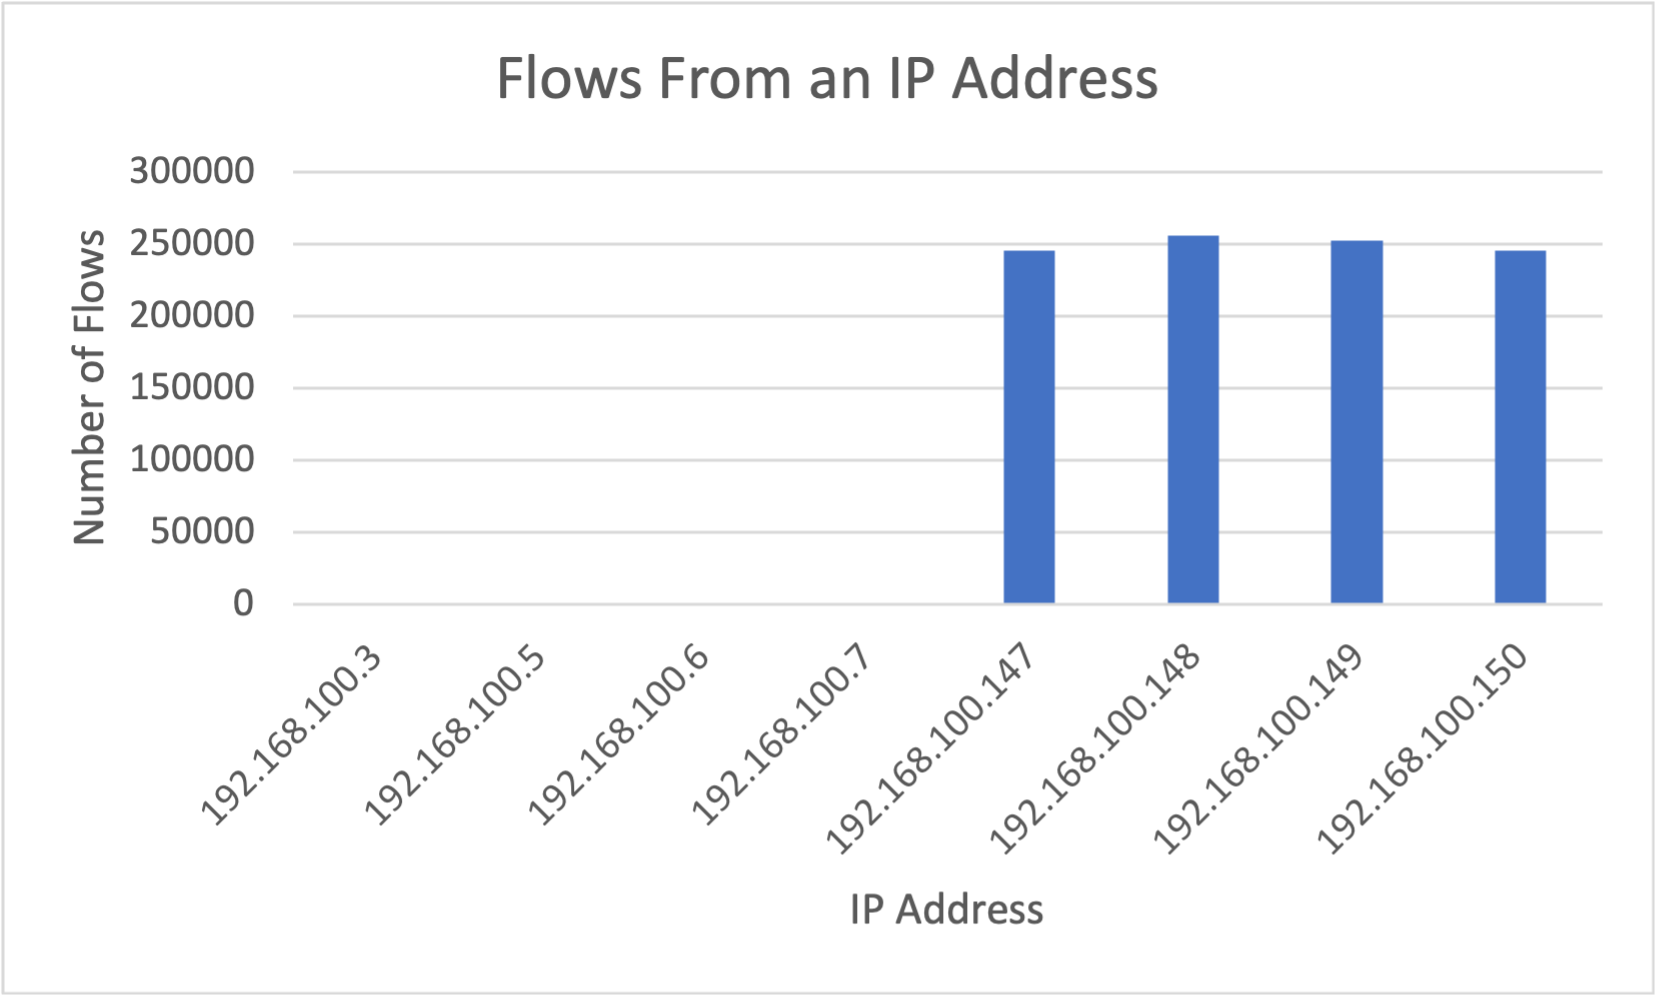
\includegraphics[width=8cm]{Figure1.png}
    \centering
    \caption{The number of flows that were sent from particular IP addresses}
    \label{fig:flowfrom}
\end{figure}

\begin{figure}[htbp]
    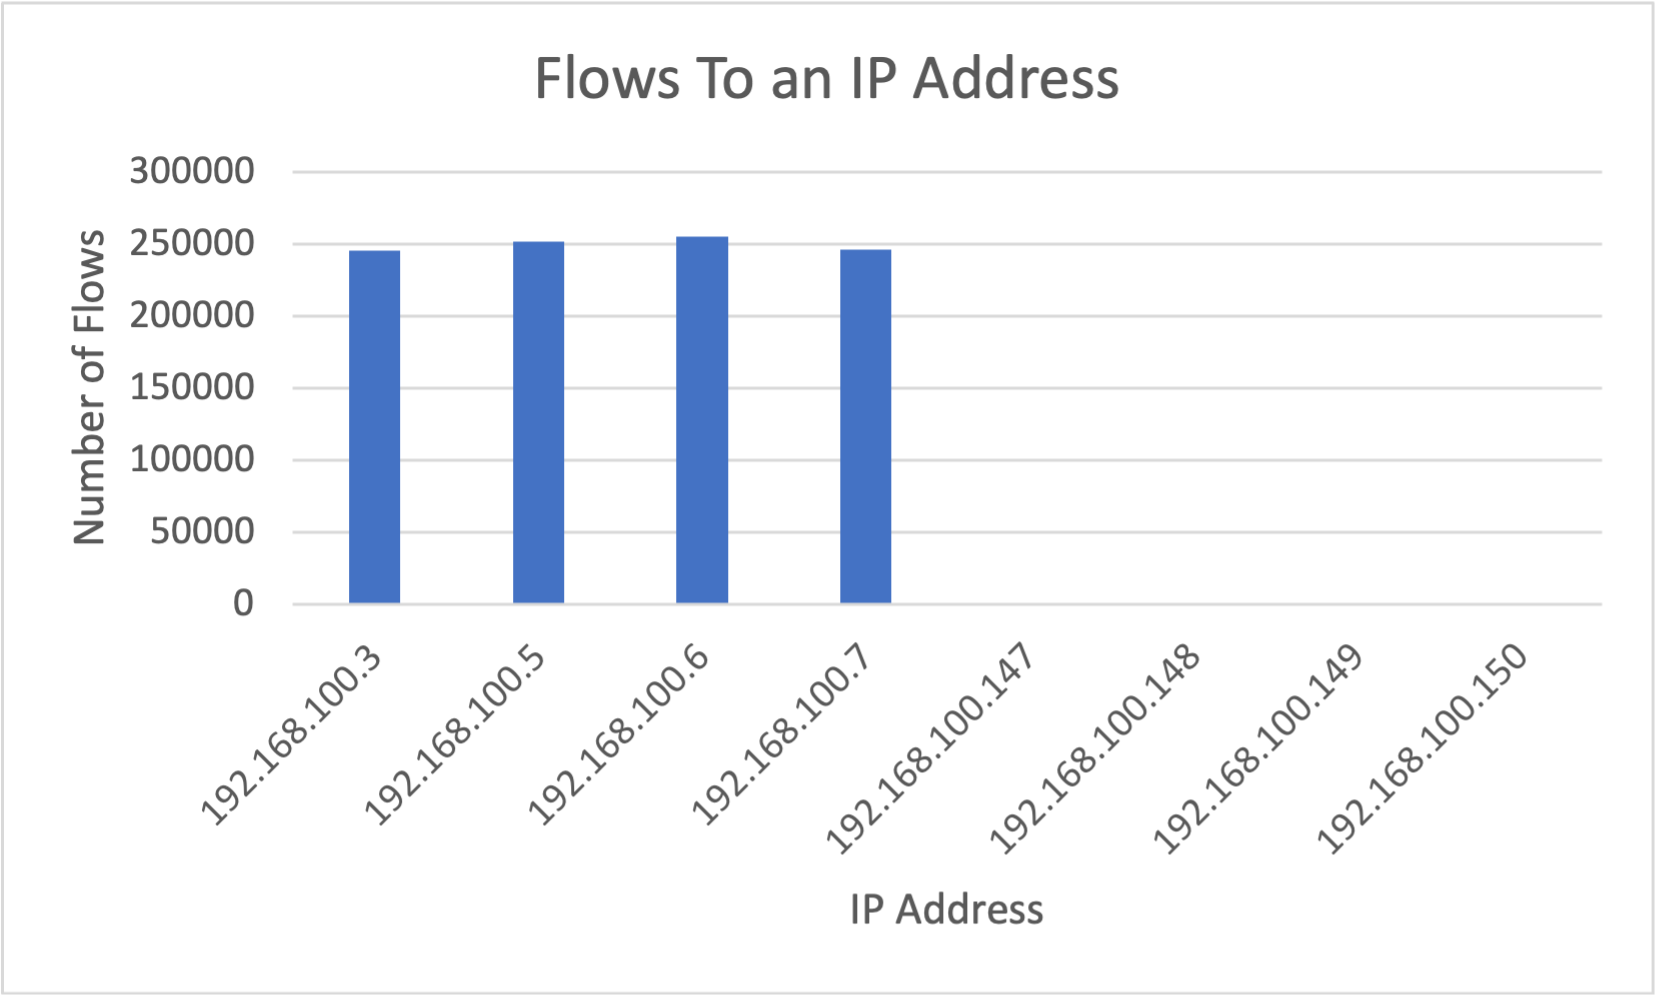
\includegraphics[width=8cm]{Figure2.png}
    \centering
    \caption{The number of flows that were sent to particular IP addresses}
    \label{fig:flowto}
\end{figure}

A clear pattern of sending and receiving was being established in the data. The IP addresses that were sinks had hundreds of thousands
of flows going into them whereas the sources had 285 at the highest. If one were to look at the flows coming out the
relationship is opposite. These features could be potential indicators of some sort of attack whether DDoS,
Network Scanning or otherwise. To determine this further, the average number of flows per second was determined as
shown in figures \ref{fig:sentfrompersec} and \ref{fig:senttopersec}. This was gained in a similar fashion to figure 
\ref{fig:flowfrom} and \ref{fig:flowto} with dividing them further based on their Unix time stamp and making an average.

While it is good to see how much data was being sent overall, it doesn't really tell very much about what's happening.
In order to determine something like a DDoS attack, the average packets sent pers second was determined to be more useful.

\begin{figure}[htbp]
    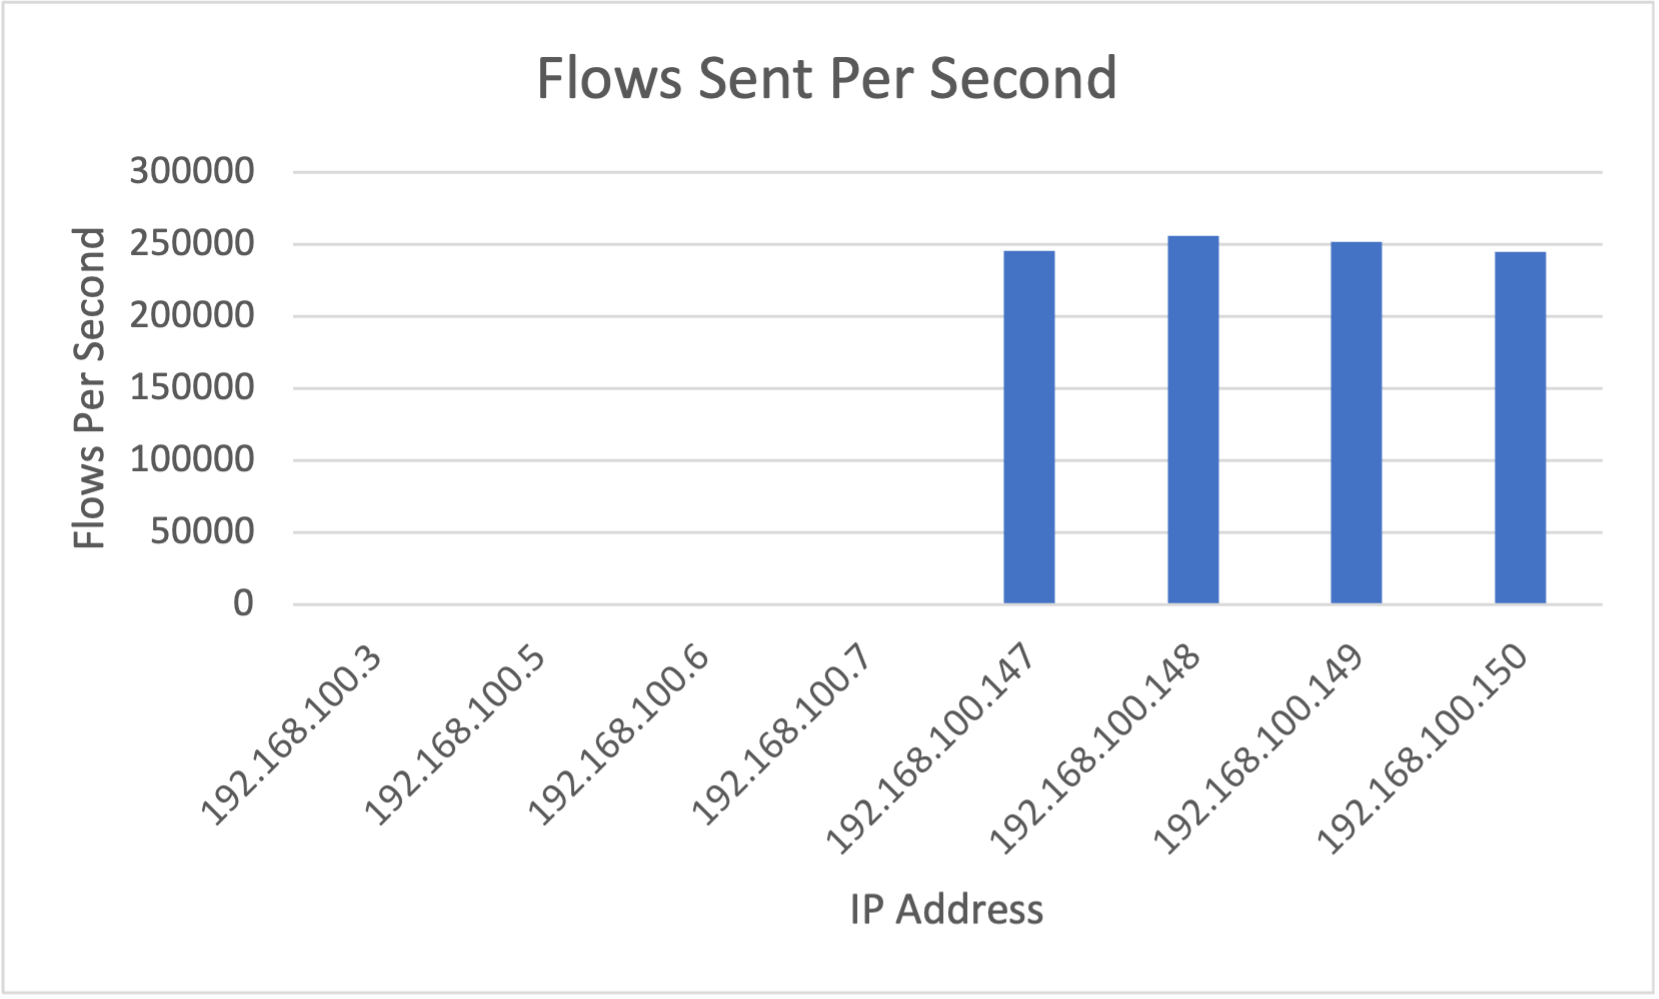
\includegraphics[width=8cm]{Figure3.png}
    \centering
    \caption{The number of flows that were sent from particular IP addresses per second}
    \label{fig:sentfrompersec}
\end{figure}

\begin{figure}[htbp]
    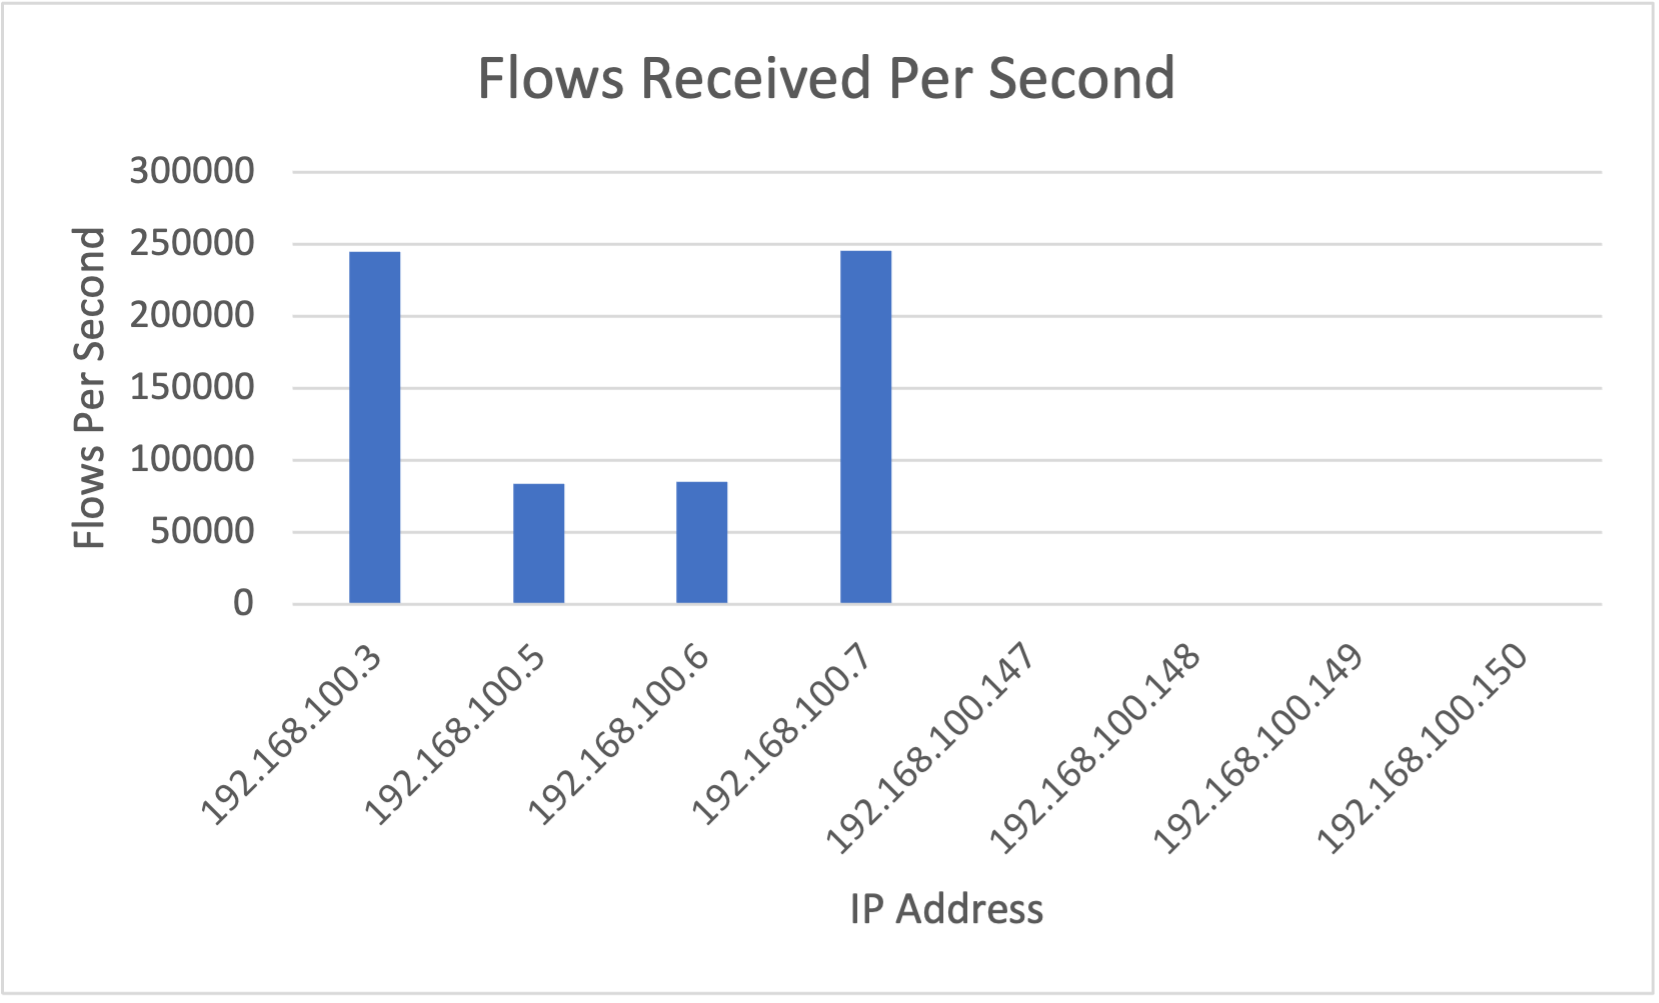
\includegraphics[width=8cm]{Figure4.png}
    \centering
    \caption{The number of flows that were sent to particular IP addresses per second}
    \label{fig:senttopersec}
\end{figure}

As with figures \ref{fig:flowfrom} and \ref{fig:flowto}, these figures also showed clear trends with definitive
sinks and sources. Like before, the sinks have hundreds of thousands of flows received per second whereas the sources
send hundreds of thousands of flows per second. However this was not enough to fully determine what was going on with
this data. To make a more definitive conclusion the number of ports each IP address contacted was found as shown in 
figure \ref{fig:portscontacted}. 

\begin{figure}[htbp]
    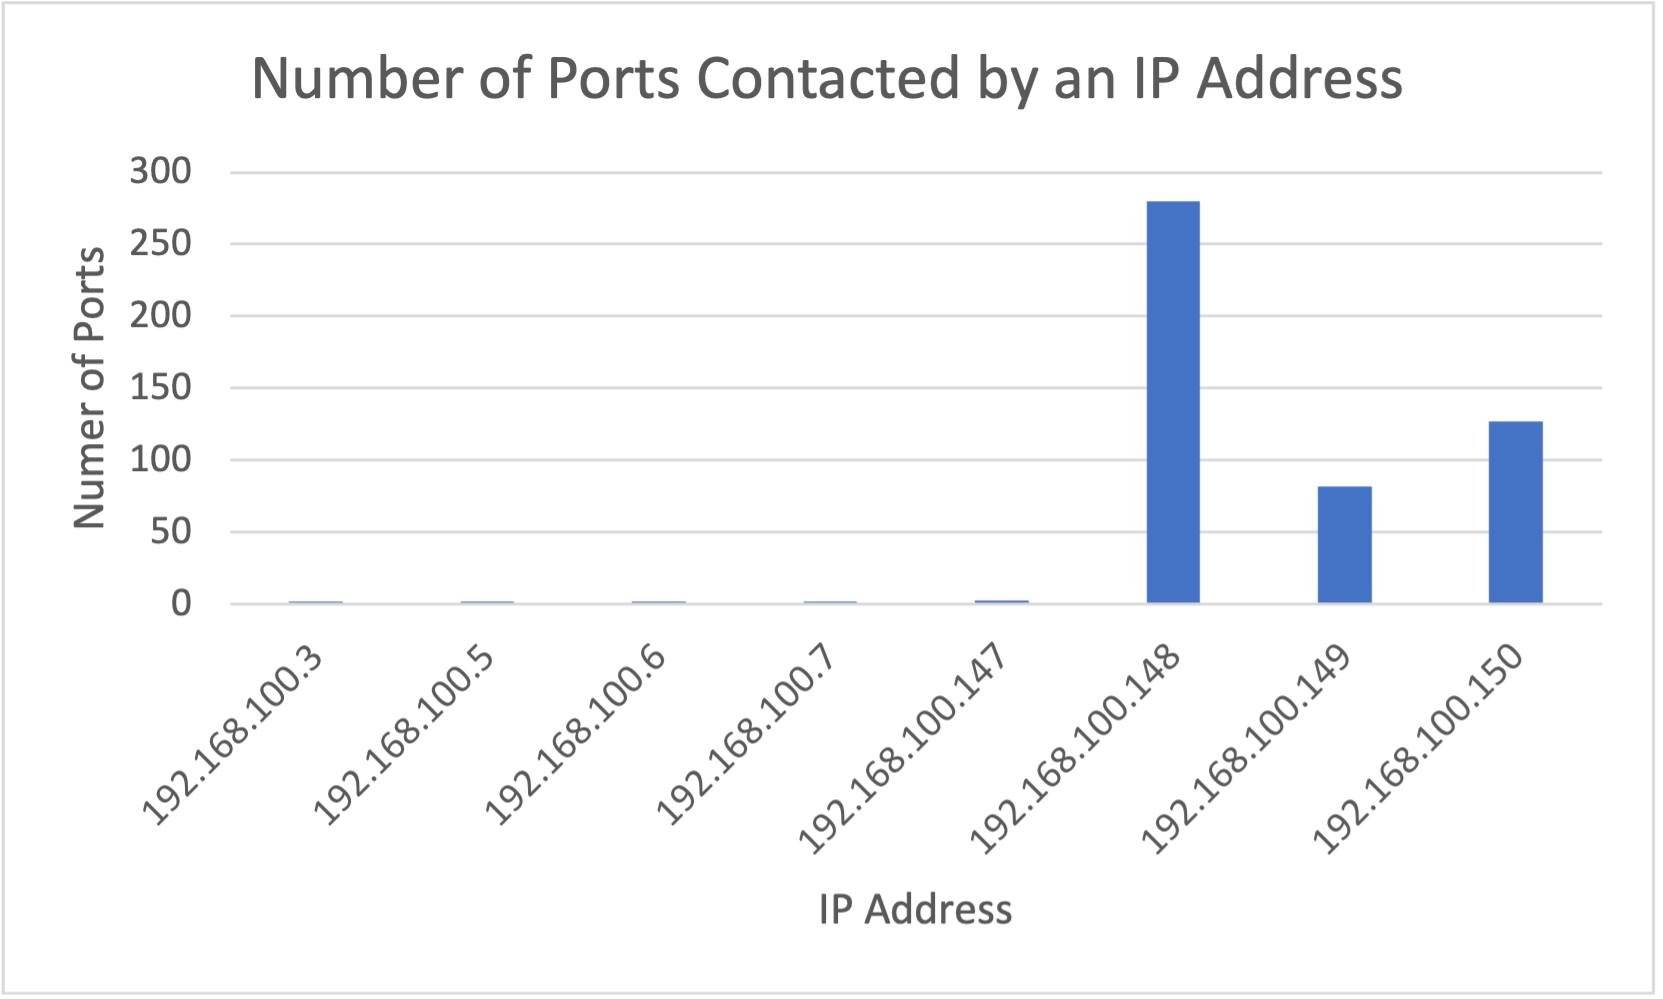
\includegraphics[width=8cm]{Figure5.png}
    \centering
    \caption{The number of ports contacted per IP address}
    \label{fig:portscontacted}
\end{figure}

This figure provided a more definitive idea about what was going on for some of the IP Addresses. This query
 was performed by counting the unique ports contacted by each IP address. In order
to determine whether a network scan had occured, one must look at the number of ports contacted on a particular
device within quick succession in a particular timeframe. If it is an abnormally high number, it is likely a 
network scan attack has occurred. In particular, 192.168.100.148 contacted the most ports at 280 ports total 
being contacted likely indicating that it was performing a network scan on one of the other networks. 
Similarily could be said for 192.168.100.149 and 192.168.100.150 with less confidence at 82 and 127 ports
contacted respectively.

With the question of network scans out of the way, the last question remained.
Was it possible that any of the sinks were being DDoSed?
For a DDoS to occur there should be an odd number of incoming, unique, flows to a particular IP address. 

\begin{figure}[htbp]
    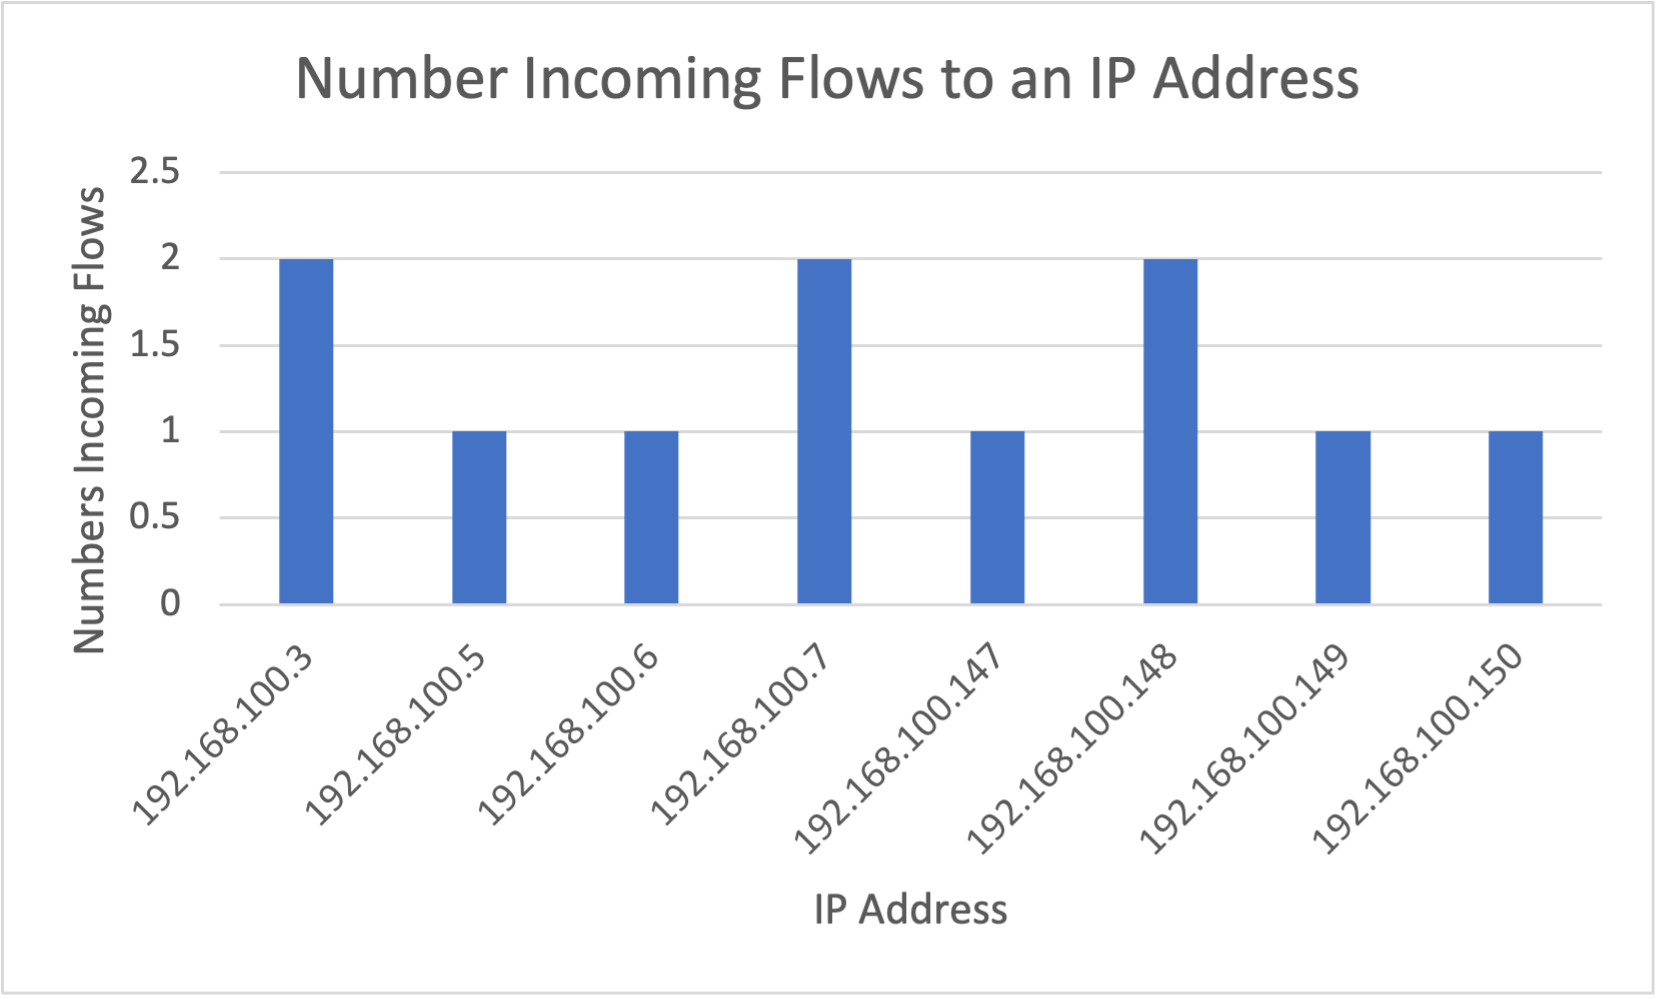
\includegraphics[width=8cm]{Figure6.png}
    \centering
    \caption{The number of flows from unique IP addresses coming into a particular IP address}
    \label{fig:incomingflows}
\end{figure}

As shown in figure \ref{fig:incomingflows} there are very few flows to any device. This query
was performed by looking at the unique nodes that connected to the IP addresses. All devices in this sample have 
only one or two connections. In order to determine if a DDoS attack had occured within a timeframe, what would have
to be looked for is an abnormally large number of flows coming into a device in order for it to be considered
distributed. Without it, there is no proper way of determaning Denial of Service from flow data alone. 
Thus, there is no evidence that any DDoS attacks occured withing this timeframe, ruling out a DDoS attack as a source 
of the flows to the IoT device. 

\section{Discussion and Future Work}

Clearly the work done here is just the beginning, however the results already gained show great promise of revealing
important information. From so little data and simple queries we can already get a good idea about whether two 
important attacks occur in a matter of seconds. From data such as flows per second and unique devices connecting it is possible to figure 
out if a DDoS attack is occuring. From data such as ports contacted it is possible to see if the network is being
scanned. The results thus far are promising about a future for this project, however the results found by these
queries on this dataset are limited. For one, only simple queries were and more advanced queries could and should 
be used in the future in order to solve more complicated problems and answer more complicated questions. Secondly, 
the fraction of the dataset used only involved 1,000,000 flows. In order to get a more accurate picture of a network, 
millions more flows so be gathered and analyzed. Luckily, due to the speed of graph databases, this shouldn't be a 
problem for similar experiments in the future. There are so many doors and paths the author was not able to take 
during this project due to various limitations and constraints. 

Expanding the queries performed to answer more complicated questions was one such work that the author was not able 
to conduct during the writing of this paper. However, such work would be very useful in order to gain more analytics
to answer questions including, but certainly not limited to, detecting patterns in the flows where it is seen how 
often flows are sent and if they appear targeted more to one device rather than another. 

Additional work should be done to analyze these basic questions at scale, whether that be scale of time or scale of 
data. The very small sample of data only encompased a few seconds of flow traffic with only six IP Addresses being
monitored. For a true, real-world test of this system, timeseries data spanning minutes, hours, or even days should 
be used. In addition, a more fleshed out, small network testbed should be used with a greater sample of IoT devices. 
There are many limitations and challanges on this especially with the papers stated goal of being useful for homes and
small networks. Such limitations and challanges revolve around the processing power and storage space required to
analyze and store such data. However, that is precicely what makes this an optimal work to determine better the 
feasability of using such systems on home and small networks.

To add onto this, more work also needs to be performed on the comparison of the utility of graph databases for these 
tasks in comparison to more traditional methods as well as the benefits and/or downfalls to increasing efficiency of 
the existing systems for these tasks. Due to limitations and constraints involved with this project, very little
benchmarking was performed, especially as it pertains to comparisons towards relational database management systems.
Future work should be focused on this topic so as to obtain definitive data comparing the two options as well as what
relational database systems truly do better or worse on in comparison to graph database systems with regards to
the specific questions related to IoT timeseries data. 

\section{Conclusion}
While there are many avenues this work could take in the future, the goal that this paper set out with was
achieved. It was shown that graph databases could effectively use IoT timeseries data to answer questions
that would be of interest to both home and small network users. It has been shown that graph databases work
on timeseries databases with relatively simple queries to produce results for real world applications such
as determining attacks on certain devices within a network. The future work mentioned before is both proper
and necessary for taking this project forward. It is the hope of the author the the findings and questions
found in this paper prove of use to future research and future projects and that the findings, whatever they
may be, lead to more efficient use of timeseries data for IoT devices.

\printbibliography

\end{document}